% Unified video-presentation slides covering the full paper.
% Two presenters: Aksan (slides 1-9, ~5:30 min) and Mahbubur (slides 10-17, ~5:00 min).
% Total target time: ~10:30 minutes.
% Compile with: pdflatex slides.tex (twice if you add cross-references).

\documentclass[aspectratio=169,11pt]{beamer}

\usetheme{metropolis}
\usepackage{graphicx}
\usepackage{booktabs}
\usepackage{xcolor}
\usepackage{array}

\definecolor{accent}{HTML}{1E64C8}
\definecolor{warn}{HTML}{C81E1E}
\setbeamercolor{progress bar}{fg=accent}
\setbeamercolor{frametitle}{bg=accent}

\title{Parameter-Efficient Adaptation of SAM~2 for\\Sentinel-1 SAR Flood Inundation Mapping\\in the Indo-Gangetic Region}
\author{Aksan Gony Alif \and Mahbubur Rahman}
\institute{BRAC University}
\date{}

\begin{document}

% ====================================================================
% PART 1 - Aksan: motivation, methods, datasets, setup (~5:30 min)
% ====================================================================

% ---------------------------------------------------------- Slide 1
\maketitle

% ---------------------------------------------------------- Slide 2
\begin{frame}{Why this paper exists}
\begin{itemize}
    \item Bangladesh floods every monsoon. \emph{Cloud cover} makes optical satellites unreliable when flood maps matter most.
    \item Sentinel-1 SAR \textbf{penetrates clouds}, available globally and free.
    \item But SAR is a noisy, single-channel, logarithmic-intensity signal, nothing like the natural RGB photographs vision foundation models (SAM, SAM 2) are pretrained on.
    \item \textbf{Question:} can we adapt SAM 2 to radar, \emph{cheaply}, and have it generalize to an unseen flood event?
\end{itemize}
\vspace{0.5em}
\textbf{Answer (preview):} yes, mostly, with one important caveat about the cross-polarization channel.
\end{frame}

% ---------------------------------------------------------- Slide 3
\begin{frame}{Three gaps in prior work}
\begin{enumerate}
    \item[\textbf{1.}] \textbf{No head-to-head comparison} of parameter-efficient fine-tuning (PEFT) methods on SAM-family backbones for SAR floods. Prior papers use one method each; you can't tell which adapter to pick.
    \vspace{0.5em}
    \item[\textbf{2.}] \textbf{No test of operational utility} of uncertainty estimates. Prior SAR-flood work reports aggregate calibration (low ECE) but does not test whether the resulting \emph{per-pixel} scores are useful for triage.
    \vspace{0.5em}
    \item[\textbf{3.}] \textbf{No public reproducible OOD test set} combining temporal \emph{and} geographic out-of-distribution shift on Sentinel-1. Standard benchmarks hold out one country, but all events are from 2017--2019.
\end{enumerate}
\vspace{0.5em}
\centering
\emph{We close all three.}
\end{frame}

% ---------------------------------------------------------- Slide 4
\begin{frame}{Methodology: a controlled empirical sweep}
\textbf{5 backbones $\times$ 4 PEFT methods $\times$ 3 seeds}
\begin{center}
\small
\begin{tabular}{lcccc}
\toprule
Backbone & LoRA & DoRA & Conv-LoRA & AdaptFormer \\
\midrule
SAM ViT-B (94 M)            & \checkmark & \checkmark & \checkmark & \checkmark \\
SAM 2 Hiera-B+ (81 M)       & \checkmark & \checkmark & \checkmark & \checkmark \\
\addlinespace[0.3em]
SAM ViT-L (308 M)           &           &           & \checkmark &            \\
SAM ViT-H (636 M)           &           &           & \checkmark &            \\
SAM 2 Hiera-L (224 M)       &           &           & \checkmark &            \\
\bottomrule
\end{tabular}
\end{center}
\vspace{0.5em}
\begin{itemize}
    \item Full sweep + baselines: $\approx$ \textbf{3.5 hours}, $\approx$ \textbf{\$10} cloud compute (dual NVIDIA RTX PRO 5000 Blackwell).
    \item Uncertainty: \textbf{Monte Carlo dropout}, 20 stochastic passes per chip.
\end{itemize}
\end{frame}

% ---------------------------------------------------------- Slide 5
\begin{frame}{Polarimetric ``pseudo-RGB'' input}
SAM 2 was pretrained on three RGB channels. Sentinel-1 gives us only two:
\begin{itemize}
    \item \textbf{VV} (co-polarization): vertical transmit, vertical receive.
    \item \textbf{VH} (cross-polarization): vertical transmit, horizontal receive.
\end{itemize}
We must synthesize a third channel.
\vspace{0.8em}

\textbf{Three compositions compared:}
\begin{center}
\small
\begin{tabular}{ll}
\toprule
\textbf{ratio} & $(\,\text{VV},\;\text{VH},\;10 \log_{10}(P_{VV}/P_{VH})\,)$ \\
\textbf{diff}  & $(\,\text{VV},\;\text{VH},\;\text{VV}_{dB} - \text{VH}_{dB}\,)$ \\
\textbf{single} & $(\,\text{VV},\;\text{VV},\;\text{VV}\,)$ \\
\bottomrule
\end{tabular}
\end{center}
\vspace{0.6em}

\small
By the dB-domain identity $10\log_{10}(P_{VV}/P_{VH}) = \text{VV}_{dB} - \text{VH}_{dB}$, \emph{ratio} and \emph{diff} produce identical model inputs. The meaningful contrast is between dual-polarization (ratio or diff) and single-polarization (VV alone).
\end{frame}

% ---------------------------------------------------------- Slide 6
\begin{frame}{Four evaluation splits}
\begin{center}
\small
\begin{tabular}{lcl}
\toprule
\textbf{Split} & \textbf{Chips} & \textbf{Role} \\
\midrule
Sen1Floods11 test       & 90  & In-distribution (10 countries) \\
Sen1Floods11 Bolivia    & 15  & Held-out country \\
Pakistan-S1F11 subset   & 12  & Regional in-distribution (2010 event) \\
\textcolor{accent}{\textbf{Pakistan-2022}} & \textcolor{accent}{\textbf{39}} & \textcolor{accent}{\textbf{Strict OOD: new geography + time}} \\
\bottomrule
\end{tabular}
\end{center}
\vspace{0.6em}
\begin{itemize}
    \item The first three splits come from \textbf{Sen1Floods11} (Bonafilia et al., CVPR Workshops 2020). All events are from 2017--2019.
    \item The fourth, \textbf{Pakistan-2022}, is constructed in this work. It covers the August--September 2022 Indo-Gangetic monsoon flood, the same meteorological system that produces Bangladesh's annual flooding.
\end{itemize}
\end{frame}

% ---------------------------------------------------------- Slide 7
\begin{frame}{Pakistan-2022 dataset construction}
\textbf{Two public sources, paired in this work:}
\begin{itemize}
    \item \textbf{Labels:} TU Wien Sentinel-1-derived flood-extent product\\ (Roth et al., NHESS 2023; CC-BY 4.0)
    \item \textbf{Imagery:} Microsoft Planetary Computer \texttt{sentinel-1-rtc}\\ (Radiometric Terrain Corrected, anonymous SAS-token access)
\end{itemize}
\vspace{0.6em}

\textbf{Pipeline:} for each TU Wien mask date, find the matching Sentinel-1 RTC scene, read at native 10\,m, reproject the mask upward to 10\,m, tile into 512$\times$512 chips.

\vspace{0.6em}
\textbf{Result:} 39 chips at native 10\,m, fully Sen1Floods11-compatible layout.

\vspace{0.4em}
\textcolor{warn}{\emph{Acquisition note:}} the first chip set was at 20\,m and mismatched the training distribution. We rebuilt at native 10\,m; that is the dataset released here.
\end{frame}

% ---------------------------------------------------------- Slide 8
\begin{frame}{Experimental setup}
\textbf{Training protocol:}
\begin{itemize}
    \item 10 epochs on the 252 Sen1Floods11 hand-labelled training chips.
    \item AdamW optimizer; separate learning rates $10^{-4}$ (adapters) / $10^{-5}$ (unfrozen pretrained weights); cosine schedule with 200-step linear warmup.
    \item Loss: Dice + binary cross-entropy with logits, equal weight.
    \item Mixed-precision fp16; batch size 1 with gradient accumulation 4 (effective batch 4).
    \item \textbf{No training-time data augmentation.} Test-time augmentation (4 rotations $\times$ 2 flips = 8 views) is applied only at inference for the ensemble condition.
\end{itemize}
\vspace{0.4em}
\textbf{Seeds:} 42, 123, 20025 (three independent reruns per cell).
\end{frame}

% ---------------------------------------------------------- Slide 9 (handoff)
\begin{frame}{From setup to findings}
\centering
\vspace{0.4em}
\textbf{\large The next half: what we actually found.}\\[1em]
Across the four evaluation splits, plus one diagnostic finding we did \emph{not} expect:\\[1.2em]
\textcolor{warn}{\large The cross-polarization channel turns out to be the operative\\out-of-distribution failure mode.}
\end{frame}

% ====================================================================
% PART 2 - Mahbubur: results, diagnostic, conclusion (~5:00 min)
% ====================================================================

% ---------------------------------------------------------- Slide 10
\begin{frame}{Headline results}
\begin{center}
\small
\begin{tabular}{lcccc}
\toprule
Method & Sen1F11 test & Bolivia & Pak-S1F11 & Pak-2022 \\
\midrule
U-Net baseline                & 0.601 & \textbf{0.684} & 0.271 & \textbf{0.672} \\
Hiera-B+ + AdaptFormer        & \textbf{0.634} & 0.458 & 0.254 & \textcolor{warn}{0.090} \\
Hiera-B+ + LoRA               & 0.599 & 0.635 & 0.255 & \textcolor{warn}{0.140} \\
Hiera-B+ + DoRA               & 0.602 & 0.637 & 0.254 & \textcolor{warn}{0.132} \\
\bottomrule
\end{tabular}
\end{center}
\vspace{0.6em}
\begin{itemize}
    \item \textbf{In-distribution:} AdaptFormer wins ($0.634$), beating U-Net at a fraction of trainable parameters.
    \item \textbf{Bolivia held-out:} DoRA matches U-Net ($0.637$ vs $0.684$).
    \item \textbf{Pakistan-2022:} every SAM-family cell collapses to \textcolor{warn}{$0.09$--$0.14$}, while U-Net retains $0.672$.
\end{itemize}
\end{frame}

% ---------------------------------------------------------- Slide 11
\begin{frame}{The Pakistan-2022 collapse: not a backbone or adapter problem}
\begin{itemize}
    \item Every SAM-family cell collapses, regardless of:
    \begin{itemize}
        \item Backbone (ViT-Base, ViT-Large, ViT-Huge, Hiera-Base-Plus, Hiera-Large, all collapse)
        \item PEFT method (LoRA, DoRA, Conv-LoRA, AdaptFormer, all collapse)
        \item Random seed
    \end{itemize}
    \item U-Net on the same training data does not collapse. So the collapse is \emph{specific to the adapted SAM-family models}, not a property of the dataset.
    \item \textbf{Question:} what is the SAM family seeing that the U-Net is not?
\end{itemize}
\end{frame}

% ---------------------------------------------------------- Slide 12
\begin{frame}{The polarimetric ablation: cross-polarization is the culprit}
\begin{center}
\small
\begin{tabular}{lcc}
\toprule
Pakistan-2022 IoU & Dual-polarization & Single-polarization (VV only) \\
\midrule
Hiera-B+ Conv-LoRA & $0.113$ & $\mathbf{0.632 \pm 0.057}$ \\
Hiera-B+ LoRA      & $0.144$ & $\mathbf{0.631 \pm 0.050}$ \\
Hiera-B+ DoRA      & $0.131$ & $\mathbf{0.658 \pm 0.014}$ \\
Hiera-B+ AdaptFormer & $0.092$ & $\mathbf{0.556 \pm 0.050}$ \\
\midrule
\emph{U-Net reference} & \multicolumn{2}{c}{$0.672$} \\
\bottomrule
\end{tabular}
\end{center}
\vspace{0.6em}
\textbf{Drop the cross-polarization (VH) channel and the collapse vanishes.}
\begin{itemize}
    \item Single-polarization Pakistan-2022 IoU jumps to $0.56$--$0.66$ across three seeds.
    \item Within $0.01$--$0.12$ of the U-Net baseline.
    \item \textbf{Three-seed evidence; no overlap with the dual-pol band.}
\end{itemize}
\end{frame}

% ---------------------------------------------------------- Slide 13
\begin{frame}{Qualitative comparison: same chip, three predictions}
\begin{center}
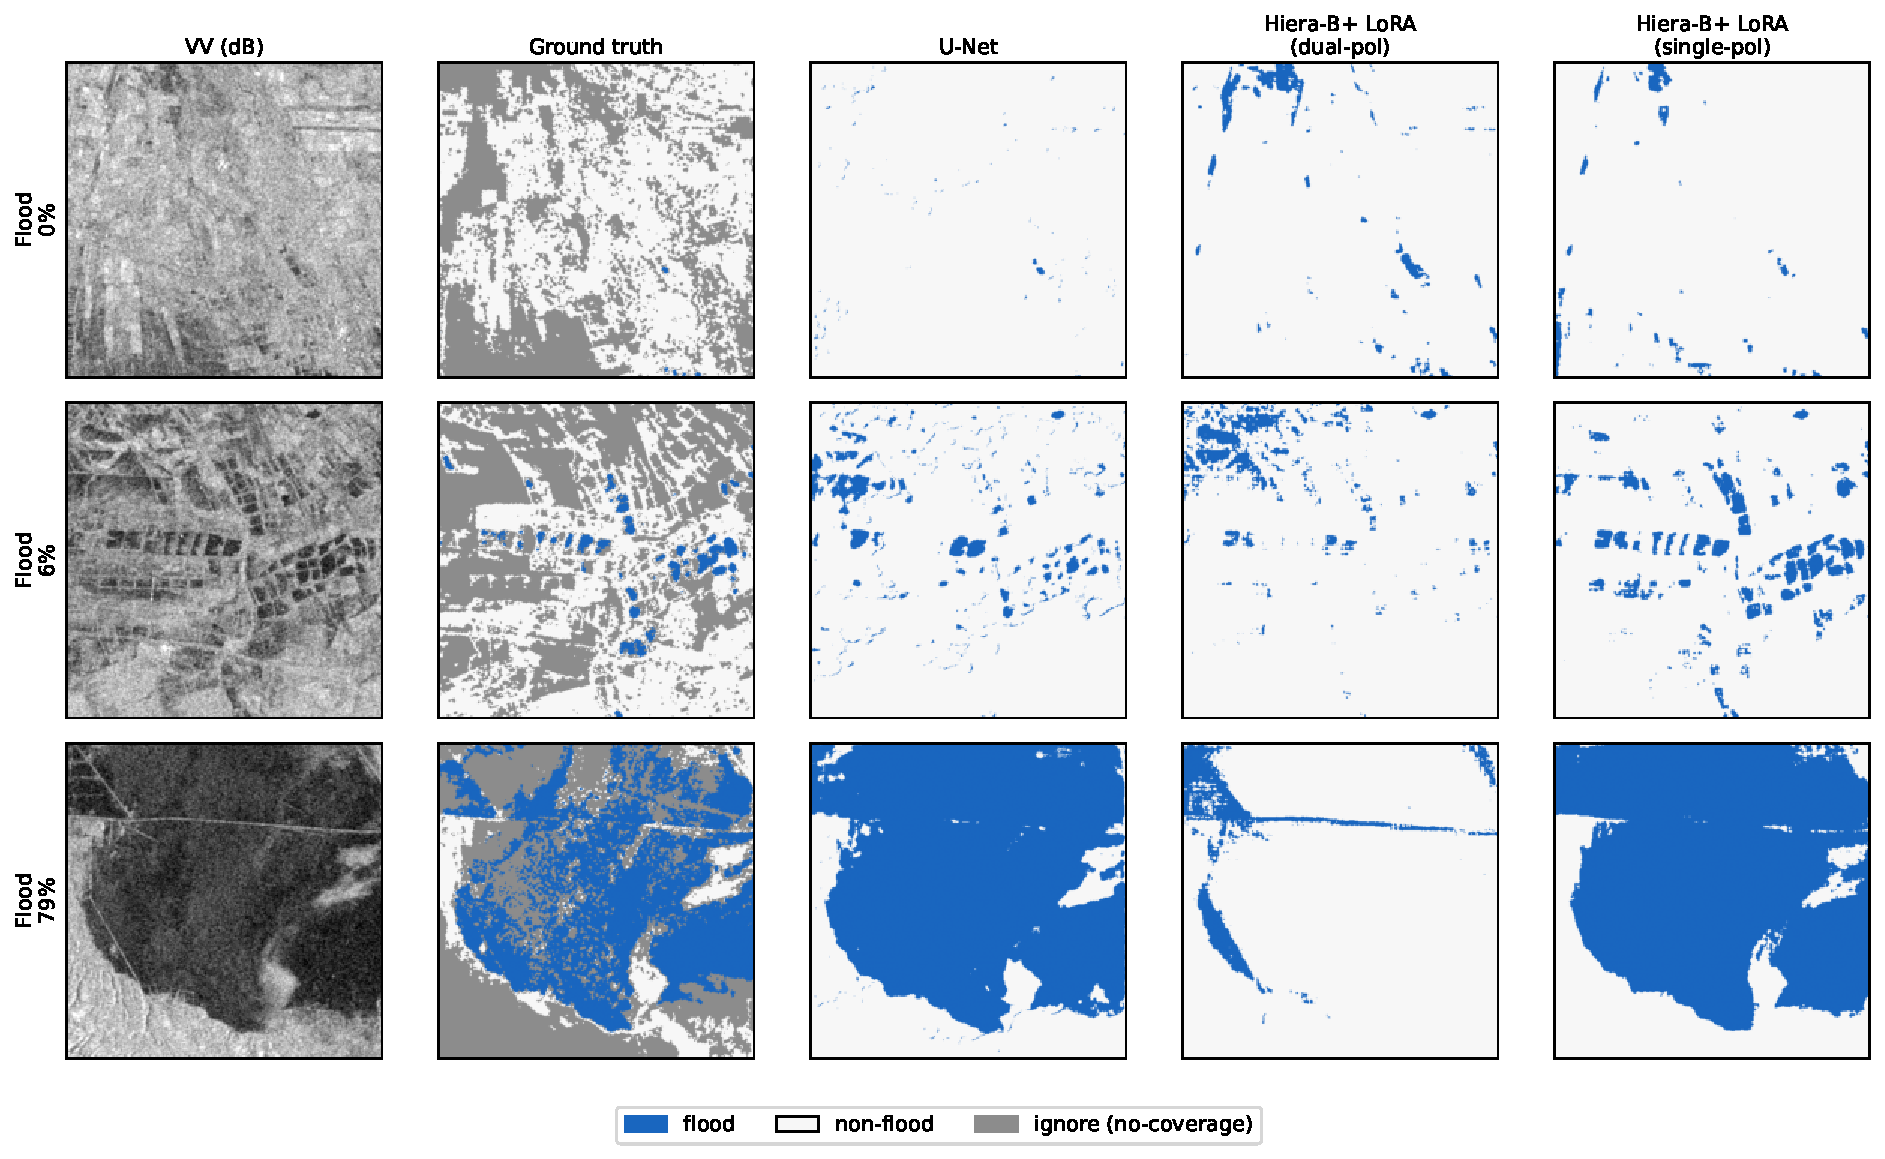
\includegraphics[width=\linewidth]{../figs/pakistan2022_overlay.pdf}
\end{center}
\vspace{0.4em}
\small
Three Pakistan-2022 chips spanning $0.2\%$, $6\%$, and $79\%$ flood fraction. Columns: VV intensity, ground truth, U-Net, Hiera-B+ LoRA dual-pol, Hiera-B+ LoRA single-pol.
\end{frame}

% ---------------------------------------------------------- Slide 14
\begin{frame}{Why? The transformer amplifies cross-polarization distribution shift}
\begin{itemize}
    \item The cross-polarization channel \emph{helps} in-distribution. Its marginal statistics on Pakistan-2022 differ from Sen1Floods11.
    \item Possible drivers: different scattering geometry, different surface conditions, different acquisition mode parameters.
    \item The SAM transformer's global attention \emph{amplifies} this distribution shift.
    \item The U-Net's local receptive fields \emph{tolerate} it.
\end{itemize}
\vspace{0.6em}
\textbf{Operational recommendation:} for new regions or events, abstain from the cross-polarization channel. Use VV only.
\end{frame}

% ---------------------------------------------------------- Slide 15
\begin{frame}{Negative finding: MC dropout is not per-pixel useful on OOD}
\textbf{Aggregate calibration is fine:}
\begin{itemize}
    \item ECE = $0.053$ on in-distribution test (at the well-calibrated threshold).
    \item ECE = $0.067$ on Pakistan-2022 (essentially unchanged despite the IoU collapse).
\end{itemize}
\vspace{0.6em}

\textbf{But pointwise selective-prediction curves are flat:}
\begin{itemize}
    \item Abstaining on the most uncertain pixels does \emph{not} improve IoU on the remaining ones.
    \item Aggregate calibration $\nRightarrow$ per-pixel difficulty ranking on OOD events.
    \item Contradicts the implicit assumption in prior SAR-flood uncertainty work.
\end{itemize}
\end{frame}

% ---------------------------------------------------------- Slide 16
\begin{frame}{Three gaps, three closures}
\begin{enumerate}
    \item[\textbf{1.}] \textbf{PEFT comparison:} controlled head-to-head; accuracy-versus-generalization trade-off documented. AdaptFormer maximizes in-distribution IoU; LoRA family is more generalization-robust.
    \vspace{0.6em}
    \item[\textbf{2.}] \textbf{Calibration vs operational utility:} substantive negative finding. Aggregate ECE does not imply per-pixel uncertainty utility on OOD.
    \vspace{0.6em}
    \item[\textbf{3.}] \textbf{Public OOD test set:} Pakistan-2022 (39 chips, native 10\,m) released with acquisition pipeline.
\end{enumerate}
\vspace{0.6em}
\textbf{Bonus diagnostic finding:} cross-polarization is the operative OOD failure mode for SAM-family adapters.
\end{frame}

% ---------------------------------------------------------- Slide 17
\begin{frame}{Limitations and future work}
\textbf{Honest limitations:}
\begin{itemize}
    \item Pakistan-2022 evaluation rests on 39 chips and TU Wien labels derived from a Sentinel-1 model.
    \item Stretch backbones evaluated only under Conv-LoRA.
    \item Bangladesh-Sylhet construction pipeline is released, chips are not yet built or evaluated.
\end{itemize}

\textbf{Future work:}
\begin{itemize}
    \item Empirical evaluation on the Bangladesh-Sylhet test set.
    \item Characterize the cross-polarization shift directly (incidence angle, acquisition mode).
    \item Sharper uncertainty estimators: deep ensembles, learned reject heads.
\end{itemize}
\vspace{0.6em}
\begin{center}
\Large \textbf{Thank you.}\\
\small \emph{Questions?}
\end{center}
\end{frame}

\end{document}
